\paragraph{ISA-VIZ1: An executable multi-resolution (Z128) interface demo.}
We include a concrete ``centerwired'' Hilbert decoder (adapted from the Z128 stable-sector framework) that compiles each codon under $\mu^\ast$ to $(N,w,V,\Delta)$ and treats the three $m=6$ boundary words as a minimal control alphabet gating local refinement to $m\in\{8,10\}$.
\begin{figure}[H]
\centering
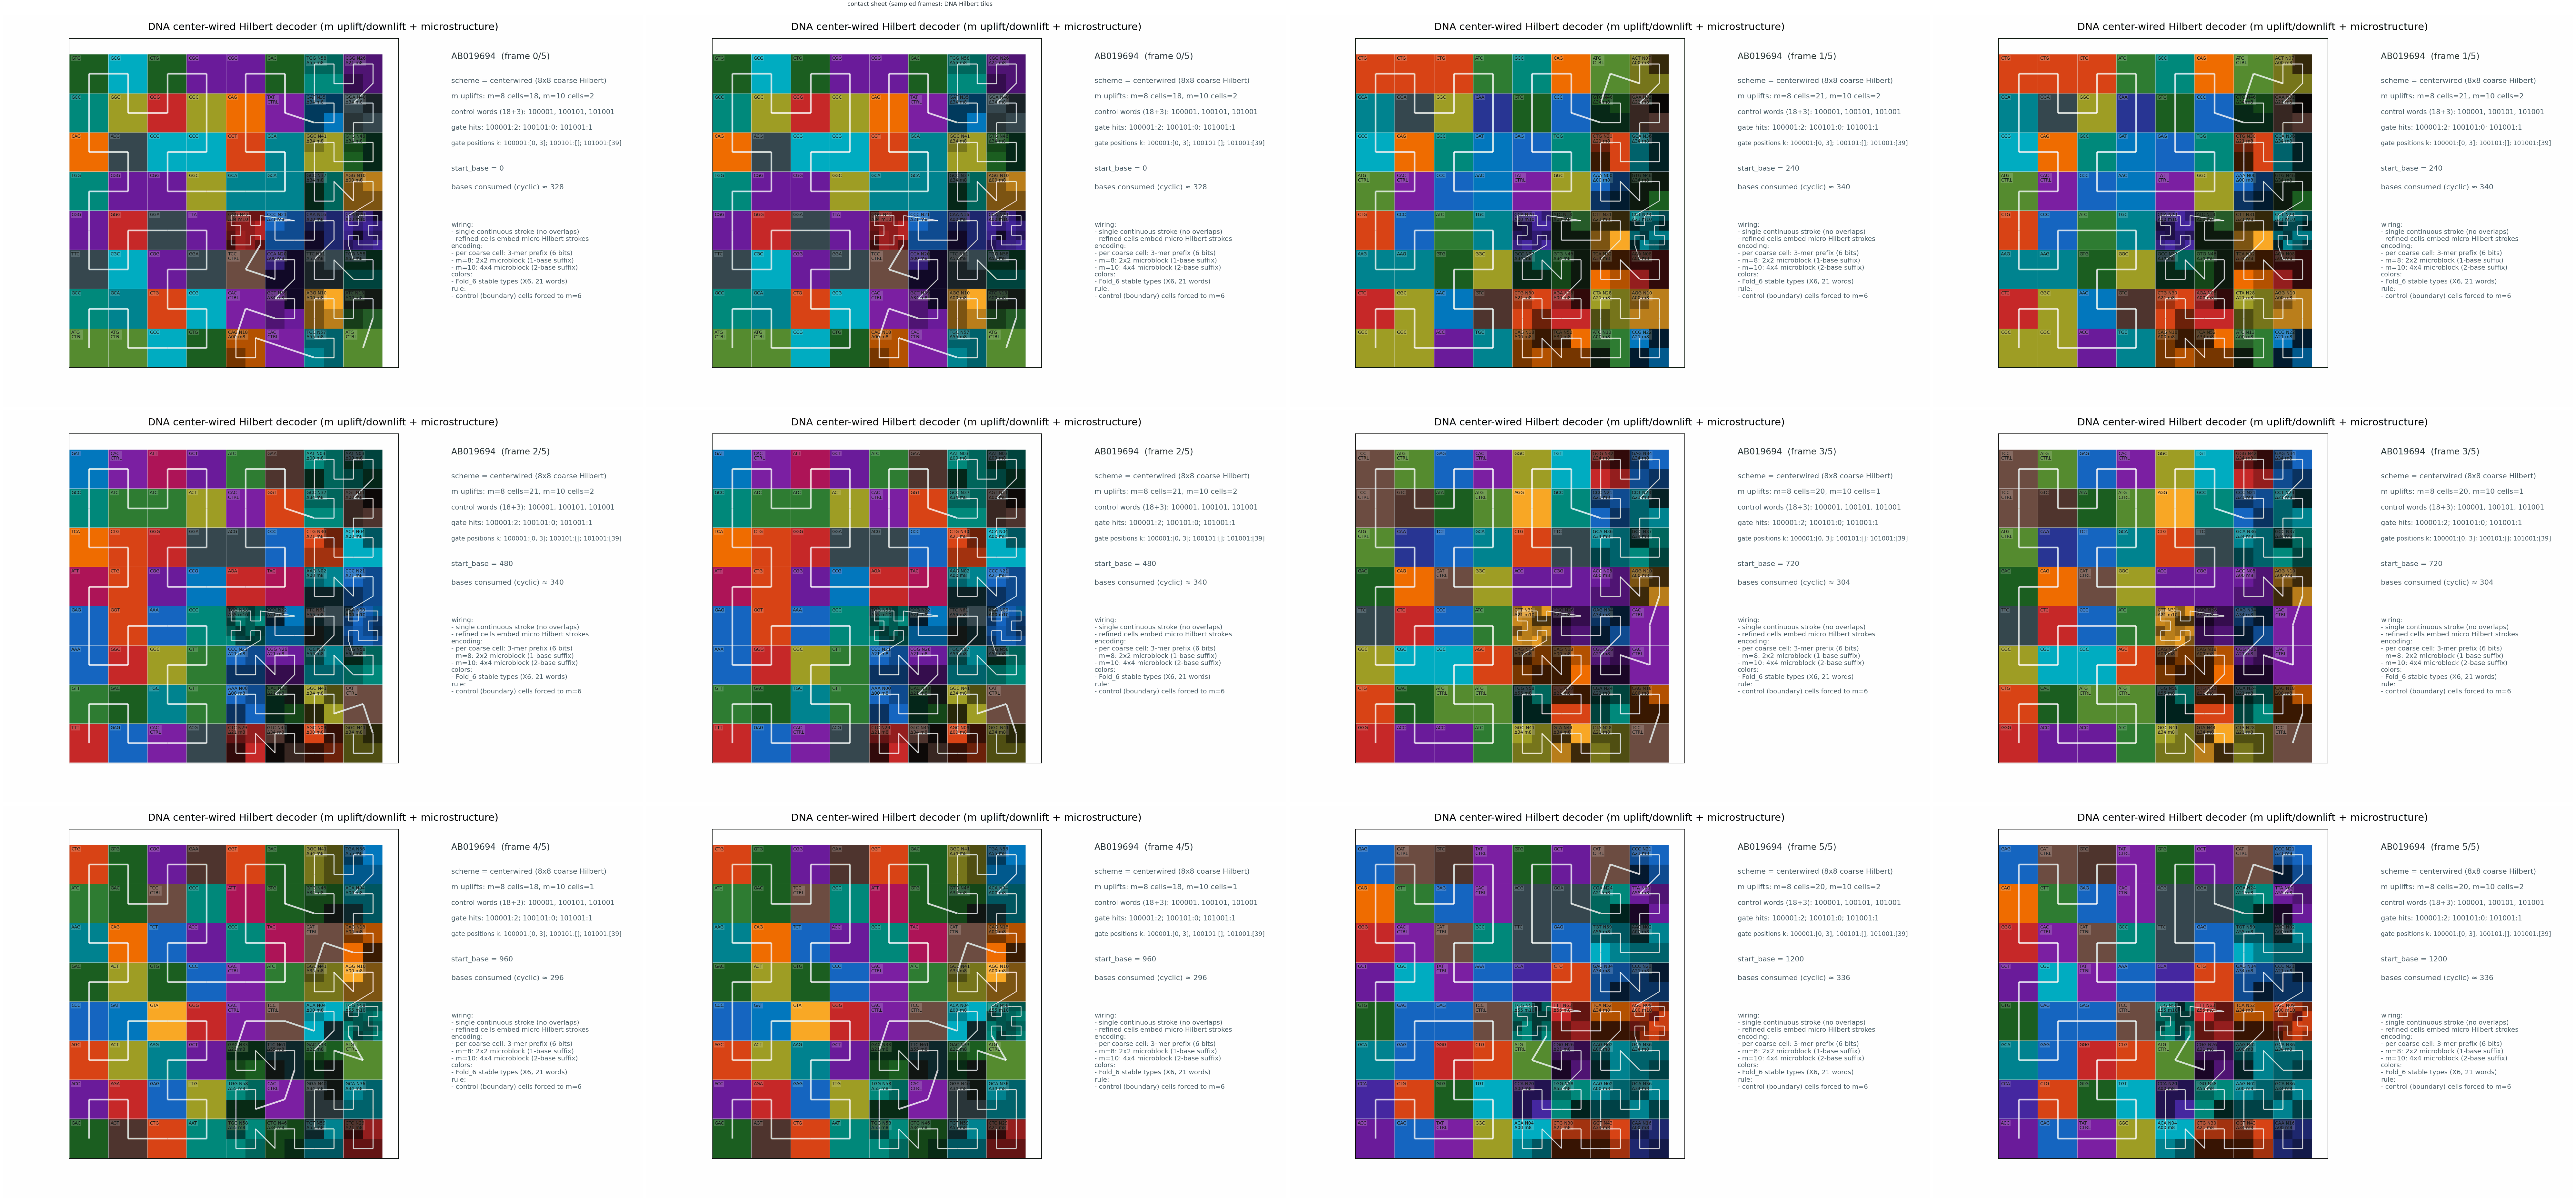
\includegraphics[width=0.98\linewidth]{figures/ab019694_centerwired_gates_contact_sheet.png}
\caption{Centerwired decoder demonstration on \path{AB019694.1} (Sec example).
Each coarse cell consumes a 3-mer prefix ($m=6$), colored by its Fold$_6$ stable type; the three boundary words $\{\texttt{100001},\texttt{100101},\texttt{101001}\}$ are treated as control records (thick border) that gate a local refinement schedule. Inside refined mode, payload cells display microstructure as embedded Hilbert strokes ($m=8$: 1-base suffix; $m=10$: 2-base suffix for selected $\Delta$ values). This is a visualization convention illustrating how an $m=6$ Hilbert screen can carry local $m=8/m=10$ information; it is not used as evidence for the biological endpoints.}
\label{fig:centerwired_decoder_demo}
\end{figure}
\noindent\textbf{Legend:} \path{figures/ab019694_centerwired_gates_legend.png}.
